\documentclass[11pt,oneside]{report}
\usepackage[utf8]{inputenc}
\usepackage{graphicx}
\usepackage[german]{babel}
\usepackage{blindtext}
\usepackage{graphicx}
\graphicspath{ {./images/} }
\usepackage{float}
\usepackage{listings}
\lstdefinestyle{code}{
	basicstyle=\footnotesize,
	captionpos=b,
	frame=single,
	keepspaces=true,
	showspaces=false,
	showstringspaces=false,
	showtabs=false,
	tabsize=2
}
\usepackage{geometry}
 \geometry{
 a4paper,
 left=30mm,
 right=15mm,
 top=20mm,
 bottom=40mm,
 }
\usepackage{helvet}
\renewcommand{\familydefault}{\sfdefault}
\renewcommand{\baselinestretch}{1.5}


\begin{document}

\begin{titlepage}
    \begin{center}
        \vspace*{1cm}
            
        \Huge
        \textbf{Maschinelles Lernen}
            
        \vspace{0.5cm}
        \LARGE
        als Projektarbeit im Informatikunterricht
            
        \vspace{1.5cm}
            
        \textbf{Jonas Groß-Hartmann}
            
        \vfill
        
        \Large
        Fach: Informatik\\
        Fachlehrer: Herr Boettcher\\
        Datum: 11.03.2024
            
    \end{center}
\end{titlepage}


\setcounter{page}{2}
\tableofcontents

\listoffigures

\newpage


\section{Einführung}
KI ist zu einem sehr wichtigem Bestandteil unserer Gesellschaft geworden. Es stehen Chat-Bots wie ChatGPT zur verfügen, welche Texte zu jedem beliebigem Thema in jeder beliebigen Art in jeder Sprache schreiben können. Es gibt KIs zur Bildgenerierung wie Midjourney, welche Bilder in Sekunden generieren können, für die Künster Wochen brauchen. KI wird ein immer größerer Teil unseres Alltages, da immer mehr große Firmen KI-Features in ihre Produkte einbauen. Viele Handys haben beispielsweise Funktionen, mit denen man Teile aus Bildern ausschneiden kann und das der Hintergrund mithilfe einer KI anschließend ausgefüllt wird.

Maschinelles Lernen ist ein Teilgebiet der KI. Man kann durch dieses Gebiet eigene erste KI-Projekte erstellen und testen. Es ist also ein guter Einstieg in die KI. Daher habe ich mich dazu entschieden, in diesem Gebiet meine Facharbeit zu schreiben und in dem Prozess mein erstes KI-Programm zu erstellen. Da ich allerdings nur Low-End-Computer zur Verfügung habe, möchte ich mich dabei auch auf die Performanz des Programm konzentrieren und ein relativ gutes Modell entwickeln, ohne dabei eine sehr lange Zeit auf Ergebnisse warten zu müssen.


\chapter{Theoretische Grundlagen}

\section{Maschinelles Lernen}
Maschinelles Lernen ist eines der wichtigsten Teilgebiete der Künstlichen Intelligenz.\footnote{Schmid, Ute (2022): Maschinelles Lernen, URL: https://www.bidt.digital/glossar/maschinelles-lernen/, Stand: 29.01.2024} Unter Maschinellem Lernen (englisch: Machine Learning) versteht man einen Vorgang, bei dem ein System automatisch Muster und Zusammenhänge aus Daten erkennt und sich mit der Zeit verbessert, ohne dabei explizit programmiert worden zu sein. Daher wird Maschinelles Lernen häufig in Wirtschaft, Forschung und Entwicklung verwendet. Man kann dabei Werte vorhersagen, Wahrscheinlichkeiten berechnen, Gruppen und Zusammenhänge in Daten erkennen, Dimensionen ohne großen Informationsverlust reduzieren und Geschäftsprozesse optimieren.\footnote{vgl. Wuttke, Laurenz (2023): Machine Learning: Definition, Algorithmen, Methoden und Beispiele, URL: https://datasolut.com/was-ist-machine-learning/ , Stand: 29.01.2024}

\subsection{Funktionsweise}
Bei Maschinellem Lernen wird einem Modell Informationen gegeben. Dieses Programm erkennt nun Zusammenhänge und Muster zwischen den Eingabewerten und gibt daraufhin einen Wert aus. Dafür wird dem Modell zunächst als Training ein Datenset übermittelt, mit dem es trainiert wird. Dabei überprüft sich das Modell selbst, da mit den Daten auch die gewünschte Zielvariable übermittelt wird. Nachdem das Modell trainiert wurde werden ihm neue, unbekannte Daten übermittelt mit deren Hilfe das Modell nun Vorhersagen treffen kann. Es findet also keine Programmierung im klassischen Sinne statt, da das Programm sich selbst trainiert und programmiert.\footnote{ebd.}

\subsection{Arten des Machine Learnings}
Es gibt vier verschiedene Arten von Maschinellem Lernen, welche verschieden Strategien verwenden und daher verschiedene Anwendungsbereiche abdecken.

%\subsubsection{Überwachtes Lernen}
Das überwachte Lernen (eng.: Supervised Learning) verwendet bekannte Daten, um aus diesen zu lernen. Der Algorithmus erkennt dabei einen Zusammenhang zwischen den Eingabedaten und der Zielvariable. Dies wird zum Beispiel zur Klassifikation und zur Vorhersage von Daten verwendet.

%\subsubsection{Unüberwachtes Lerne}
Das unüberwachte Lernen (eng.: Unsupervised Learning) dagegen hat keine vorgegebenen Zielvariable. Das Modell erkennt hier selbstständig zusammenhänge zwischen den Eingabedaten und gibt diese als Gruppen aus. Daher wird dies zur Clusteranalyse („Eine Clusteranalyse ist ein exploratives Verfahren, um Datensätze hinsichtlich ihrer Ähnlichkeit in Gruppen einzuteilen“\footnote{Wuttke, Laurenz (2022): Clusteranalyse einfach erklärt, URL:https://datasolut.com/wiki/clusteranalyse/, Stand: 02.03.2024}) und zur Dimensionsreduktion verwendet.

%\subsubsection{Teilüberwachtes Lernen}
Das teilüberwachte Lernen (eng.: Semi-Supervised Learning) ist eine Mischung aus über- wachtem und unüberwachtem Lernen, da hier eine geringe Menge an Daten mit Zielvariable und eine große Menge ohne Zielvariable genutzt werden. Dadurch werden weniger bekannte Daten benötigt, was häufig kostengünstiger und weniger Arbeitsintensiv ist, da Daten meist manuell einer Zielvariable zugewiesen werden müssen.

%\subsubsection{Verstärkendes Lernen}
Das verstärkende Lernen (eng.: Reinforcement Learning) verfolgt eine andere Idee des Machine Learnings. Das Programm hat keinen Trainingsdatensatz, es belohnt und bestraft sich durch verschiedene Handlungen mithilfe einer Kostenfunktion. Der Algorithmus weiß also nicht, was die richtige Handlung ist. Er versucht, ein Ziel zu erreichen und dabei die Kosten, welche durch die Kostenfunktion bestimmt werden, möglichst klein zu halten.

Da in dieser Arbeit ein Programm zur Bilderklassifizierung erstellt wird, wird ein Modell mit überwachtem Lernne verwendet. Dies wird meistens zur Klassifizierung von Daten, wie beispielsweise Bildern, verwendet. Daher wird auch ein Datensatz mit beschrifteten Bildern benötigt.\footnote{vgl. Wuttke(2023)}


\section{Neuronale Netzwerke}
Ein Grundbestandteil des Machine Learnings und von KI generell ist das künstliche neuronale Netz. Mit diesem kann ein Modell aus Daten entscheiden, was der jeweilige Output ist. Ein künstliches neuronales Netz ist einem Nervensystem nachempfunden. Daher hat es einen sehr ähnlichen Aufbau.

\subsection{Neuronen}
Ein Netz besteht aus mehreren Neuronen. Diese haben meist mehrere Inputs und einen Output. Im menschlichen Körper heißen die Inputs Dendriten und der Output Axon und funktionieren wie ein künstliches Neuron. Die Inputs erhält das Neuron dabei meist von anderen Neuronen und gibt Outputs an andere Neuronen weiter. Dadurch entsteht ein Netz aus vielen, zusammenhängenden Neuronen.

\subsection{Aufbau eines Neuronalen Netzes}
Ein Neuronales Netz besteht aus mehreren Schichten, sogenannte „Layer“. Diese Layer bestehen aus beliebig vielen Neuronen, welche mit den Neuronen des vorherigen und des folgenden Layers verbunden sind. Dabei gibt es drei Arten von Layern. Der Input-Layer nimmt die Daten auf, die als Input übergeben werden und ist immer der erste Layer eines künstlichen Neuronalem Netz. Dementsprechent gibt es auch einen Output-Layer, welcher eine Zielvariable ausgibt. In diesem Layer gibt es immer so viele Neuronen, wie es mögliche Outputs gibt. Alle anderen Layer werden als Hidden Layers bezeichnet. Diese sind für die Verarbeitung der Daten verantwortlich. Es kann beliebig viele Hidden Layers geben und diese können beliebig viele Neuronen beinhalten. Außerdem benötigt jeder Layer eine Aktivierungsfunktion, welche bestimmt, ob ein Neuron aktiviert wird.\footnote{Welsch, Stefan (2023): Die Grundlagen neuronaler Netze - Einfach erklärt, URL: https://b-nova.com/home/content/the-basics-of-neural-networks-easily-explained/, Stand: 29.01.2024} Eine Funktion, die häufig dafür verwendet wird, ist die ReLu-Funktion (rectified linear activation function). Sie ist zur Standardaktivierungsfunktion für viele Arten von neuronalen Netzen geworden, da ein Modell, das sie verwendet, leichter zu trainieren ist und oft eine bessere Leistung erzielt.\footnote{vgl. Brownlee, Jason (2020): A Gentle Introduction to the Rectified Linear Unit (ReLU), URL: https://machinelearningmastery.com/rectified-linear-activation-function-for-deep-learning-neural-networks/, Stand: 03.03.2024}


\chapter{Technische Grundlagen}

\section{TensorFlow}
Um ein Machine Learning Modell zu entwickeln kann man verschiedene Bibliotheken und Frameworks verwenden. Ich habe mich für das Framework TensorFlow in Python entschieden, welches für das erstellen von Maschine Learning Modellen gut geeignet ist. Auf der offiziellen Website von TensorFlow sieht man, dass die Bibliothek von vielen großen Firmen genutzt wird wie beispielsweise Google, Coca-Cola und Intel.\footnote{vgl. https://www.tensorflow.org/about/case-studies, Stand: 02.03.2024}

Die Bibliothek kann mithilfe des Befehls \verb+import tensorflow as tf+ importiert werden. „\verb+as tf+“ muss dabei nicht verwendet werden, verkürzt allerdings das Aufrufen der Funktionen und wird in den meisten TensorFlow-Projekten verwendet.

\section{Keras}
Um nun ein Modell erstellen zu können wird die Keras-Bibliothek genutzt. Diese ist Teil von TensorFlow und ist eine relative Einsteigerfreundliche und einfache Software.

Mit Keras kann man ein Sequential Modell erstellen, welches der einfachste Typ eines Modells von Keras ist. Man erstellt dieses mit \verb+model = keras.Sequential()+. Als Parameter kann man nun einen Array angeben, welcher die Layers des neuronalen Netzes enthält. So kann man beispielsweise einen dense-Layer(\verb+layers.Dense(units=64, activation='relu')+) angeben. In dem Beispiel besteht der Layer aus 64 Neuronen und die Aktivierungsfunktion ist eine RuLu-Funktion.

Das Modell muss anschließend kompiliert werden. Die Methode \verb+model.compile()+ kann dafür benutzt werden. Man muss zudem einen Optimizer und eine Verlustfunktion angeben, mit denen das Modell lernt. Um die Genauigkeit des Modells anzeigen zu lassen kann man als metric-Parameter \verb+"accuracy"+ angeben, was Sinnvoll für die Bewertung des Modells ist.

Um das Modell nun zu trainieren wird die \verb+model.fit()+-Methode genutzt. Die Methode benötigt ein Trainings-Datensatz und ein Validierung-Datensatz. Das Modell wird mit dem Trainings-Datensatz trainiert, während das Validierung-Datensatz zum überprüfen des Datensatzes mit unbekannten Daten verwendet wird. Zudem muss die Anzahl der Epochen übergeben werden, die angibt, wie häufig das Modell trainiert werden soll.

Das Modell kann nun neue Daten vorhersagen mithilfe der \verb+model.predict()+-Methode. Diese benötigt als übergebenen Parameter einen oder mehrere Werte, mithilfe derer das Modell einen neuen Wert vorhersagen kann.\footnote{vgl. https://keras.io/about/, Stand: 03.03.2024}

\section{TensorFlow Lite}
Mithilfe von TensorFlow Lite kann ein fertig trainiertes Modell in einer Datei gespeichert werden, sodass sie zu einem späteren Zeitpunkt wieder aufgerufen und zur Vorhersage von Daten verwendet werden kann. Das Keras-Modell kann dadurch mithilfe folgender Methode zu einem TensorFlow Lite-Modell konvertiert werden: \verb+tf.lite.TFLiteConverter.from_keras_model(model)+. Anschleißend muss dieser Konvertiere mithilfe der Methode \verb+convert()+ das TensorrFlow Lite-Modell konvertieren. Dieses kann nun mit Standard-Pythonfunktionen gespeichert werden (\verb+with open(+ \verb+"model.tflite", 'wb') as f: f.write(tflite_model)+).

Das gespeicherte Modell kann nun jederzeit wieder aufgerufen werden, um Vorhersagen zu tätigen. Dabei muss allerdings beachtet werden, dass die Keras-Funktionen nicht mehr verwendet werden können, da es sich nun um ein TensorFlow Lite-Modell handelt. So kann nicht mehr die \verb+model.predict()+-Methode verwendet werden, da diese Teil eines Kears-Modells ist. Die entpechende Methode für das TensorFlow Lite-Modell ist \verb+classify_lite()['outputs']+. Die Methode benötigt einen Parameter, welcher der Name des Input-Layers ist, also zum Beispiel \verb+classify_lite+ \verb+(sequential_1_input=input)['outputs']+. Der Name des Input-Layers ist hier \verb+sequential_1+ und als Input wird eine Variable \verb+input+ übergeben.\footnote{vgl. https://www.tensorflow.org/tutorials/images/classification, Stand: 03.03.2024}


\chapter{Projekt}

\section{Auswählen des Datensatzes}
Um ein Modell zur Klassifizierung von Bilder erstellen zu können muss zunächst ein Datensatz ausgewählt werden. Dafür habe ich mich für einen Datensatz mit Bildern von Artikeln aus dem Supermarkt entschieden.\footnote{https://github.com/marcusklasson/GroceryStoreDataset, Stand: 10.02.2024} Der Datensatz wurde für eine andere Arbeit erstellt und steht auf der Website GitHub zu Verfügung.\footnote{Klasson, Marcus et al. (2019): A Hierarchical Grocery Store Image Dataset with Visual and Semantic Labels, URL: https://arxiv.org/abs/1901.00711, Stand: 03.03.2024} Der Datensatz wurde von mir in einen einzige Sammlung von Bildern reduziert und in der Programmierung automatisch aufgeteilt, sodass zufällig Bilder für die Modelle in Trainings- und Validierungsdatensatz aufgeteilt werden.

\section{Implementierung}
Zunächst muss der Datensatz so in einer Variable gespeichert werden, dass das Modell diesen nutzen kann. Mithilfe der Methode \verb+tf.keras.utils.image_dataset_from_directory()+ kann dies einfach getan werden. Man muss in der Methode zunächst angeben, wo die Bilder gespeichert sind, welche für den Datensatz verwendet werden sollen. In diesem Fall sind sie in einem Ordnen „\verb+food_dataset+“ im aktuellen Verzeichnis gespeichert, weshalb der Pfad folgendermaßen angegeben wird: \verb+./food_dataset+. Außerdem muss der „validation split“ angegeben werden. Dieser gibt an, wie viel Prozent der Bilder zum Überprüfen des Modells verwendet werden sollen. In diesem Fall wurde 0.1 angegeben, sodass 10\% des Datensatzes nicht im Trainingsdatensatz verwendet werden, sondern im Validierungsdatensatz. Um nun anzugeben, ob der Validierungsdatasatz oder der Trainingsdatensatz erstellt wird gibt man mithilfe des Parameters „subset“ dies an. Für den Trainingsdatensatz wird \verb+"training"+ angeben, für den Validierungsdatensatz \verb+"validation"+. Nun muss angegeben werden, auf welche Größe die Bilder skaliert werden sollen, da alle Bilder die gleiche Größe haben müssen. Hier kann ein beliebiger Wert gewählt werden, für das Modell habe ich mich für eine Höhe und Weite von 180px entschieden. Die Datensätze können nun erstellt werden und in den Variablen \verb+train_ds+ und \verb+val_ds+ gespeichert.

Als nächstes wird die Anzahl der möglichen Ergebnisse benötigt. Mithilfe der Methode der Datensätze \verb+class_names()+ kann man alle möglichen Ergebnisse in einem Array aufrufen. Die Länge dieses Arrays ist daher auch die Anzahl der Klassen.

Nun sollte man sicherstellen, dass die Datensätze während des trainieren möglichst schnell aufgerufen werden können um die Laufzeit der Trainingsphase zu minimieren. Dafür verwendet man folgende Methode: \verb+train_ds.cache().shuffle(1000).prefetch(buffer_size=AUTOTUNE)+. \verb+cache()+ hält dabei die Bilder im Speicher, nachdem sie während der ersten Epoche des Trainieren von der Festplatte geladen wurden. Dadurch werden die Bilder allerdings immer in der selben Reihenfolge aufgerufen. Um dies zu verhindern wird die \verb+shuffle()+-Methode verwendet. Durch die \verb+prefetch()+-Methode können spätere Bilder vorbereitet werden, während das aktuelle Bild verarbeitet wird. Dies verbessert häufig die Laufzeit, allerdings wird dabei auch zusätzlicher Speicher benötigt. Das Argument \verb+buffer_size+ ist für eine gute Leistung wichtig. Es wird \verb+tf.data.AUTOTUNE+ angegeben, um einen Algorithmus dafürch laufgen zu lassen, welcher einen geeigneten Wert dafür angibt.

Nun wird das Modell mithilfe der Methode \verb+tf.keras.models.Sequential()+ erstellt. Da es sich bei dem Input um Bilder handelt muss zunächst eine Kombination aus \verb+Conv2D()+-Layern und \verb+MAxPooling2D+-Layern genutzt werden.Dies ist ein Faltungsblock, welcher für die Bilderklassifizierung wichtig ist. Er besteht aus einer oder mehreren Faltungsschichten, die dazu dienen, Merkmale aus dem Eingangsbild zu extrahieren. Auf die Faltungsschichten folgen in der Regel eine oder mehrere Pooling-Schichten, die dazu dienen, die räumliche Ausdehnung der Merkmale zu verringern und gleichzeitig die wichtigsten Informationen zu erhalten.\footnote{vgl. Chatterjee, Himadri Sankar (2019): A Basic Introduction to Convolutional Neural Network, URL: https://medium.com/@himadrisankarchatterjee/a-basic-introduction-to-convolutional-neural-network-8e39019b27c4, Stand:09.03.2024} Danach werden mit einem \verb+Flatten()+-Layer die mehrdimensionellen Daten in eine Dimension komprimiert. Zusätzlich wird ein \verb+Dense()+-Layer mit 128 Neuronen zur Verarbeitung der Daten genutzt und als Output-Layer ein weiterer \verb+Dense()+-Layer mit so vielen Neuronen, wie es mögliche Klassen gibt.

Da das Modell nun erstellt und in der Variable \verb+model+ gespeichert ist kann es kompiliert werden. Der dafür genutzte Optimizer ist \verb+"adam"+, wodurch der Adam-Algorithmus verwendet wird und die \verb+tf.keras.losses.SparseCategoricalCrossentropy+-Verlustfunktion, wodurch der Kreuzentropieverlust zwischen den Klassennamen und den Vorhersagen berechnet. Zudem wird zur Bewertung des Modells der \verb+metric+-Parameter übergeben, um die Trainings- und Validierungsgenauigkeit für jede Trainingsepoche anzuzeigen.

Anschließend wird das Modell trainiert. Die Anzahl der Epochen ist dabei beliebig. Bei mehr Epochen wird die Genauigkeit größer und der Verlust kleiner, jedoch verbraucht jede Epoche Zeit. Ich habe in meinem Beispiel 20 Epochen gewählt, was bei mir insgesamt ca. 11min dauert. Mit einem besseren Laptop wäre diese Zeit jedoch kleiner.

Nun können mithilfe der Bibliothek \verb+matplotlib.pyplot+ die Trainingsergebnisse visualisiert werden.
\begin{figure}[H]
	\center
	\caption{Ergebnisse des ersten Modells mit Overfitting. Quelle: eigene Darstellung}
	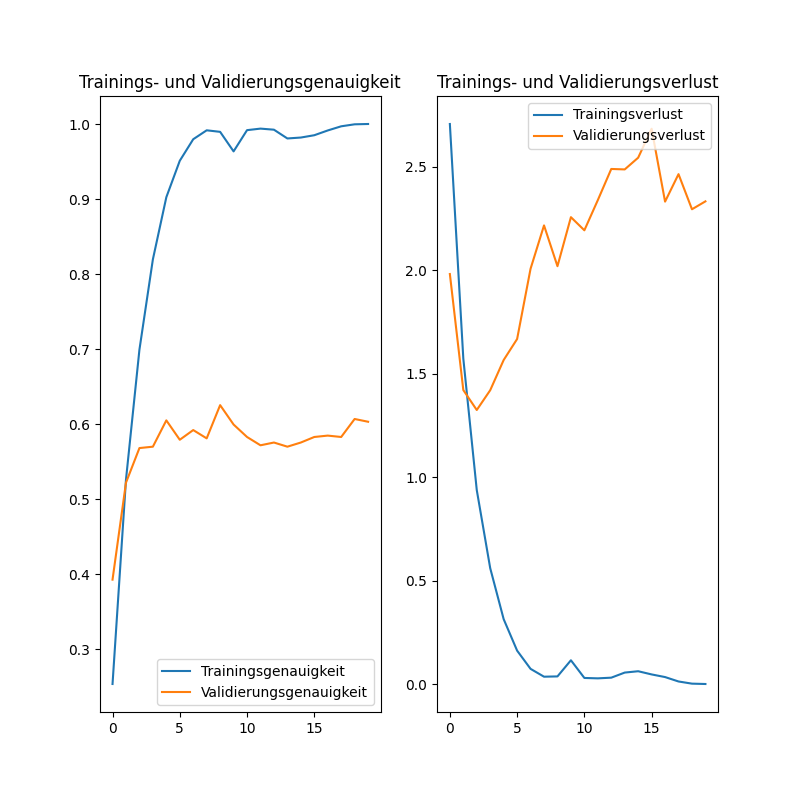
\includegraphics[width=0.5\textwidth]{model_overfitting}
\end{figure}
In Abbildung 3.1 steigt die Trainingsgenauigkeit mit der Zeit linear an, während die Validierungsgenauigkeit bei etwa 60\% im Trainingsprozess stecken bleibt. Zudem steigt der Validierungsverlust an. Dies sind Anzeichen, dass es bei dem Modell zum „Overfitting“ gekommen ist.

\section{Overfitting}
Bei einer geringen Anzahl von Trainingsbeispielen lernt das Modell manchmal aus „noise“ bzw. unerwünschten Details der Trainingsbeispiele - und zwar in einem Ausmaß, das sich negativ auf die Leistung des Modells bei neuen Beispielen auswirkt. Dieses Phänomen wird als „Overfitting“ bezeichnet. Es gibt verschiedene Wege, Overfitting entgegenzuwirken, wie beispielsweise eine Erweiterung des Datensatzes oder das zufällige Auslassen von Daten (Dropout).

\subsection{Datenerweiterung}
Overfitting tritt in der Regel auf, wenn es nur eine kleine Anzahl von Bildern gibt. Bei der Datenerweiterung werden aus den vorhandenen Bildern durch zufällige Transformationen wie Drehen, Spiegeln oder Zoomen zusätzliche Bilder erzeugt. Dies hilft dem Modell, mehr Aspekte der Daten zu berücksichtigen und besser zu verallgemeinern. Dafür wird ein zusätzliches Neuronales Netz erstellt, welches vor das hauptsächliche Neuronale Netz geschaltet wird, um den Input zu verändern. Dieses Neuronale Netz besteht aus drei Schichten: ein \verb+RandomFlip()+-Layer, ein \verb+RandomRotation()+-Layer und ein \verb+RandomZoom()+-Layer.

Der \verb+RandomFlip()+-Layer spiegelt die Bilder zufällig. Er benötigt als Argumente den Modus, welcher in diesem Fall \verb+"horizontal"+ sein sollte, wodurch die Bilder zufällig horizontal gespiegelt werden. Zudem muss das Argument \verb+input_shape+ übergeben werden, um die Dimensionen der Bilder zu definieren.

Der \verb+RandomRotation()+-Layer drecht die Bilder zufällig weit. Durch das Argument \verb+factor=0.1+ wird angegeben, das die Bilder sich maximal um \(0.1*2\pi\) drehen, da \(2\pi\) einer ganzen Kreisumdrehung entspricht.

Der \verb+RandomZoom()+-Layer kann aus Bildern herauszoomen und in Bilder hineinzoomen. Das Argument \verb+height_factor=0.1+ gibt hierbei an, dass das Bild um maximal 10\% heraus- bzw. hineingezoomt werden kann.

\subsection{Dropout}
Der Dropout kann als weiterer Layer in das Modell integriert werden, nachdem die Faltungsblöcke durchgeführt wurden. Dabei muss angegeben werden, wie viel Prozent des Inputs ausgelassen werden sollen. Wenn man dabei beispielsweise \verb+0.2+ angibt werden bei 20\% der Outputs die Aktivierung auf 0 gesetzt, wodurch Fehler ausgelassen werden können.

Nun sollte es nicht mehr zum Overfitting kommen, was man anhand der folgenden Abbildung erkennen kann.
\begin{figure}[H]
	\centering
	\caption{Ergebnisse des zweiten Modells mit Datenerweiterung und Dropout. Quelle: eigene Darstellung}
	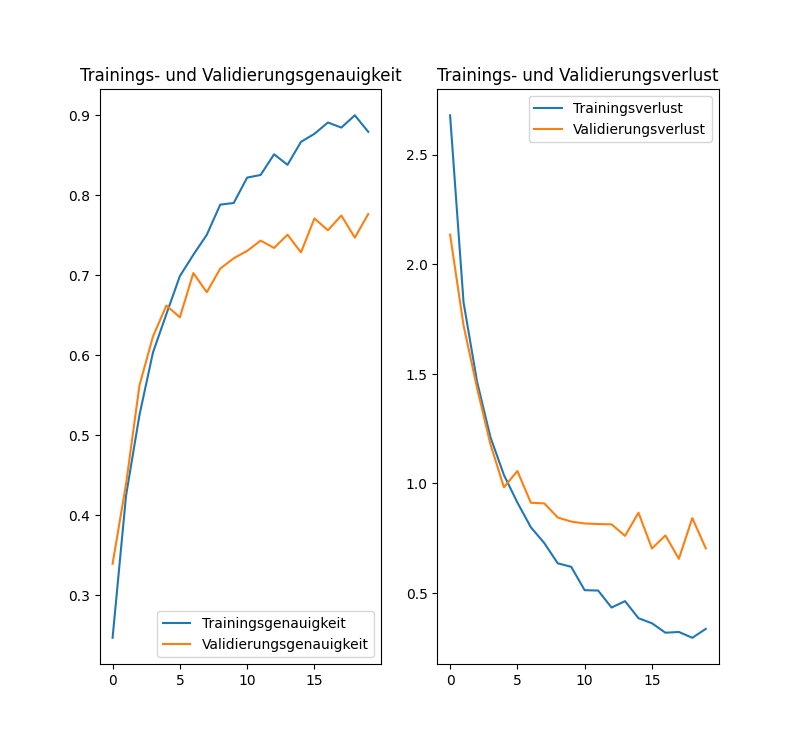
\includegraphics[width=0.7\textwidth]{model}
\end{figure}
Die Trainings- und Validierungsgenauigkeit steigen nun beide und die Validierungsgenauigkeit bliebt nicht mehr bei 60\%. Auch der Validierungsverlust sinkt nun zusammen mit dem Trainingsverlust.\footnote{vgl. https://www.tensorflow.org/tutorials/images/classification, Stand: 03.03.2024}

\section{Speichern und Aufrufen}
Das Modell kann nun mit der Methode \verb+tf.lite.TFLiteConverter.from_keras_model().convert()+ in ein TensorFlow Lite-Modell konvertiert und als solches gespeichert werden. In meinem Projekt wird es als \verb+model.tflite+-Datei gespeichert und kann nun jederzeit mithilfe der \verb+classify_lite()+-Methode aufgrufen werde. Dadurch kann man nun neue Bilder Klassifizieren. Man kann das TensorFlow-Lite-Modell nun auch auf einem Smartphone verwenden, indem man zum Beispiel eine App entwickelt. Da es sich um ein TensorFlow Lite-Modell handelt ist dieses auch sehr performant und verbraucht nicht viel Zeit und Rechenleistung.


\chapter{Fazit}
Maschinelles Lernen ist ein sehr zeitaufwendiges und ressourcenintensives Teilgebiet der Informatik und der künstlichen Intelligenz. Um auch auf Low-End-Computern ein einigermaßen gutes Modell erstellen zu können ohne sehr lange dafür warten zu müssen kann man den Datensatz auf dem Arbeitsspeicher zwischenspeichern mithilfe der \verb+cache()+-Methode 
und man kann die Anzahl der Epochen anpassen. Um schnell Daten vorhersagen zu können bzw. um schnell Bilder klassifizieren zu können kann man das Keras-Modell in ein TensorFlow-Lite Modell speichern und so sogar auf einem Smartphone aufrufen.


\appendix
\chapter{Anhang}


\lstset{style=code}

\begin{lstlisting}[language=Python]
import matplotlib.pyplot as plt
import tensorflow as tf

from tensorflow import keras
from tensorflow.keras import layers
from tensorflow.keras.models import Sequential

from datetime import date


img_height = 180
img_width = 180

train_ds = tf.keras.utils.image_dataset_from_directory(
  "./food_dataset",
  validation_split=0.1,
  subset="training",
  seed=123,
  image_size=(img_height, img_width))

val_ds = tf.keras.utils.image_dataset_from_directory(
  "./food_dataset",
  validation_split=0.1,
  subset="validation",
  seed=123,
  image_size=(img_height, img_width))

class_names = train_ds.class_names
num_classes = len(class_names)


train_ds = train_ds.cache().shuffle(1000).prefetch(buffer_size=tf.data.AUTOTUNE)
val_ds = val_ds.cache().prefetch(buffer_size=AUTOTUNE)


data_augmentation = keras.Sequential(
  [
    layers.RandomFlip("horizontal",
                      input_shape=(img_height, img_width, 3)),
    layers.RandomRotation(0.1),
    layers.RandomZoom(0.1),
  ]
)


model = Sequential([
  data_augmentation,
  layers.Rescaling(1./255),
  layers.Conv2D(16, 3, padding="same", activation="relu"),
  layers.MaxPooling2D(),
  layers.Conv2D(32, 3, padding="same", activation="relu"),
  layers.MaxPooling2D(),
  layers.Conv2D(64, 3, padding="same", activation="relu"),
  layers.MaxPooling2D(),
  layers.Dropout(0.2),
  layers.Flatten(),
  layers.Dense(128, activation="relu"),
  layers.Dense(num_classes, name="outputs")
])


model.compile(optimizer="adam",
              loss=tf.keras.losses.SparseCategoricalCrossentropy(from_logits=True),
              metrics=["accuracy"])


epochs = 20
history = model.fit(
  train_ds,
  validation_data=val_ds,
  epochs=epochs
)

acc = history.history["accuracy"]
val_acc = history.history["val_accuracy"]

loss = history.history["loss"]
val_loss = history.history["val_loss"]

epochs_range = range(epochs)

plt.figure(figsize=(8, 8))
plt.subplot(1, 2, 1)
plt.plot(epochs_range, acc, label="Trainingsgenauigkeit")
plt.plot(epochs_range, val_acc, label="Validierungsgenauigkeit")
plt.legend(loc="lower right")
plt.title("Trainings- und Validierungsgenauigkeit")

plt.subplot(1, 2, 2)
plt.plot(epochs_range, loss, label="Trainingsverlust")
plt.plot(epochs_range, val_loss, label="Validierungsverlust")
plt.legend(loc="upper right")
plt.title("Trainings- und Validierungsverlust")
plt.show()


converter = tf.lite.TFLiteConverter.from_keras_model(model)
tflite_model = converter.convert()

with open("model.tflite", "wb") as f:
  f.write(tflite_model)

\end{lstlisting}



\begin{thebibliography}{}
	\bibitem{}Brownlee, Jason (2020): A Gentle Introduction to the Rectified Linear Unit (ReLU), URL: https://machinelearningmastery.com/rectified-linear-activation-function-for-deep-learning-neural-networks/, Stand: 03.03.2024
	\bibitem{}Chatterjee, Himadri Sankar (2019): A Basic Introduction to Convolutional Neural Network, URL: https://medium.com/@himadrisankarchatterjee/a-basic-introduction-to-convolutional-neural-network-8e39019b27c4, Stand:09.03.2024
	\bibitem{}Klasson, Marcus et al. (2019): A Hierarchical Grocery Store Image Dataset with Visual and Semantic Labels, URL: https://arxiv.org/abs/1901.00711, Stand: 03.03.2024
	\bibitem{}Schmid, Ute (2022): Maschinelles Lernen, URL: https://www.bidt.digital/glossar/maschinelles-lernen/, Stand: 29.01.2024
	\bibitem{}Welsch, Stefan (2023): Die Grundlagen neuronaler Netze - Einfach erklärt, URL: https://b-nova.com/home/content/the-basics-of-neural-networks-easily-explained/, Stand: 29.01.2024
	\bibitem{}Wuttke, Laurenz (2022): Clusteranalyse einfach erklärt, URL:https://datasolut.com/wiki/clu steranalyse/, Stand: 02.03.2024
	\bibitem{}Wuttke, Laurenz (2023): Machine Learning: Definition, Algorithmen, Methoden und Beispiele, URL: https://datasolut.com/was-ist-machine-learning/ , Stand: 29.01.2024
\end{thebibliography}


\newpage

\includegraphics[width=0.9\textwidth]{selbststaendigkeitserklaerung}


\end{document}
